% Very simple template for lab reports. Most common packages are already included.
\documentclass[a4paper, 11pt]{article}
\usepackage[utf8]{inputenc} % Change according your file encoding
\usepackage{graphicx}
\usepackage{url}
\usepackage{tabularx}
\usepackage{ltxtable}
\usepackage{float}

%opening
\title{KTH H16P02 Distributed Artificial Intelligence and Intelligent Agents: Homework 2}
\author{Group 25: Fannar Magnusson (fannar@kth.se) & Thorsteinn Thorri Sigurdsson (ttsi@kth.se}
\date{\today{}}

\begin{document}

\maketitle

\section{Introduction}

For this second homework assignment we were given two tasks. The first one covered topics of communication and negotiation in a multi agent system. The task was to work further with the museum scenario and implement a Dutch Auction between an ArtistManagerAgent who is selling his work, and CuratorAgents, who are trying to get artifacts for a good price. The second task covered game mechanism design in a multi agent system where we were supposed to calculate utility/payoffs for agents and establish a Nash equilibrium for a particular situation.

\section{Tasks}

\subsection{Dutch auction for Smartmuseum}

We decided to implement an auction between one artist manager and multiple curators. The curators can be initiated with three different strategies: \textit{passive}, \textit{medium} or \textit{aggressive}. They then register their services with the Directory Facilitator Agent, indicating that they want to be participants in auctions for paintings. The artist manager is the one that initiates the auction. For that he uses a sequence behaviour. First he gets a list of all know bidders through the DF. Then he sends an \texttt{INFORM} message to them that states "start-of-auction" and contains the conversation-id used for the auction process. Now all participants should be ready for the auction. The artist manager sends a "call for proposal", setting the protocol of the message as \texttt{FIPA\_DUTCH\_AUCTION}. With the call for proposal, the artist manager sends information about the painting being auctioned and the asking price for it. The participants can get all neccessary information about the painting, such as the subject matter, paint medium and market value. The participants can be interested in different subject matters and painting mediums. If the painting being auctioned is interesting to the participant, he is willing to pay more for the painting. It depends on his bidding strategy, passive, medium or agressive, how \textbf{much} more over the market value he is willing to pay for the painting. If the participant is not willing to pay the asking price for the painting, he refuses. If the artist manager doesn't get any bids for the current asking price he decreases the asking price and calls for a new proposal. If the participant is willing to pay the asking price or more, he sends a proposal to the artist manager, saying that he is willing to pay the asking price for the painting. In that case the artist manager accepts the proposal. In the case that the artist manager doesn't get any bids that are higher or equal to the reserved price for the painting (the minimum amount the artist manager is willing to sell the painting for), he terminates the auction. If more than one participant bids on the painting, the artist manager chooses one of them to sell it to. Note that all bids will be equal, since the participants only bid the asking price for the painting, not higher, even though they would be willing to pay more. The artist manager then sends an \texttt{ACCEPT\_PROPOSAL} message to the participant that he will sell the painting to, and a \texttt{REJECT\_PROPOSAL} to all other participants that bid on the painting.

\subsubsection{Implementation}

We are using the \texttt{ContractNetInitiator} and \texttt{ContractNetResponder} behaviours to run the Dutch auction in the \texttt{ArtistManagerAgent} and \texttt{CuratorAgent}, respectively. This gives us out-of-the-box control of the auction process.

In addition to this we use a \texttt{WakerBehaviour} in the \texttt{ArtistManagerAgent} to start the auction after a certain time has passed, and a \texttt{OneShotBehaviour} to send an \texttt{INFORM} message to the bidders before starting the auction, notifying them that the auction is about to start. We use a \texttt{SequentialBehaviour} to schedule the \texttt{OneShotBehaviour} before the \texttt{ContractNetInitiator} behaviour. 

The \texttt{CuratorAgent} runs a \texttt{CyclicBehaviour} waiting for the \texttt{INFORM} message that tells him that the auction is about to start. Upon receiving that message, he starts the \texttt{ContractNetResponder} behaviour to partake in the auction.

\subsubsection{Strategies}

The curator agent needs to be initiated with one of the three differents strategies defined: \textit{passive}, \textit{medium} or \textit{aggressive}. The curator agent also has (randomly created) interests which will affect his bidding strategy. For each of the painting's attributes that matches agent's interest, his interest factor, which is initially set to \texttt{1}, is increased by \texttt{0.3}. So for example, if a particular painting has two attributes that the agent is interested in, his interest factor in the painting is \texttt{1.6}. Then depending on the curators strategy, the interest factor is multiplied by a strategy factor (\texttt{1} for passive, \texttt{1.2} for medium and \texttt{1.4} for aggressive. The outcome of this is: \texttt{interestFactor * strategyFactor = strategyMultiplier}. Now given that the curator knows the market value of the painting, he is willing to pay: \texttt{marketValue * strategyMultiplier} for the painting. 

Agents with \textit{medium} strategy will be more likely to win than agents with the \textit{passive} strategy. Agents with the \textit{aggressive} strategy will be more likely to win than the agents with \textit{medium} strategy. In addition to this there is also a random element due to the randomly generated interests.

If we have medium or aggressive curators, the auction is likely to be finished in fewer rounds since they are willing to pay more, and match the asking price sooner.

The \texttt{ArtistManagerAgent's} reserve price (lowest price he is willing to sell the painting for) is 10\% higher than the painting's market value. Therefore an agent with no interest in a painting, and a passive strategy, will never try to buy a painting, since he will only be willing to pay the market value of the painting.

\subsection{Payoff matrix and Nash equilibrium}

\subsubsection{Payoff matrix}

We assume that the curator agent has two strategies for selling paintings to profilers: a simple one and an advanced one. The simple one is quoting a price depending on overall demand. The advanced one is quoting the price depending on the profiler's interests. We assume that the advanced strategy requires more work for the curator agent and therefore results in a lower payoff when a painting is sold. Finally we assume that utility of \texttt{2} is the highest utility an agent can get, utility of \texttt{0} is neutral, and utility of \texttt{-2} is the lowest utility for an agent.

We created two payoff matrices to represent this, the first one is where the curator uses the simple strategy and the second one is where the curator uses the advanced strategy.

The values that can be read from each cell are represented like this \textit{(payoff for artist manager, payoff for curator, payoff for profiler)}. For example if we take a look at the first cell in the first table (row one, column one), we can read from it that the payoff for the \textbf{artist manager} is \texttt{1}, he made some profit of selling the high quality painting, but the profit could have been higher, like we see in the cell below where the artist manager sells a low quality painting and maximizes his profits, resulting in a payoff of \texttt{2}. If there is no sale, the artist manager gets a lower payoff if it was a high quality painting as he put more work into that one. The payoff is negative in both cases, since he is not getting paid for the work that he has done.

Now if we take a look at the payoff for the \textbf{curator agent} in the first cell of the first table, we see that it is \texttt{2}. The curator made a sale with low effort (using a simple strategy) - resulting in the highest possibly utility for him. If he sells a painting with the advanced strategy, the payoff is lower. In the case where the profiler agent doesn't buy the painting, the payoff for the curator is \texttt{-2} if he used the advanced strategy, as he put a lot of work into the sale, but the payoff is \texttt{-1} if he used the simple strategy.

If we then take a look at the payoff for the \textbf{profiler agent}, we can see that he gets a payoff of \texttt{2} when buying a high quality painting and a payoff of \texttt{1} when buying a low quality painting. However, we assume that if he doesn't buy a low quality painting, the payoff is \texttt{0} as he doesn't care about that, but if he doesn't buy a high quality painting, the payoff is \texttt{-1} as he will be disappointed to have missed the opportunity to buy the painting.

%\LTXtable{\textwidth}{payoff_matrix_demand_table.tex}
%\LTXtable{\textwidth}{payoff_matrix_interest_table.tex}

\begin{figure}[h]
    \centering
    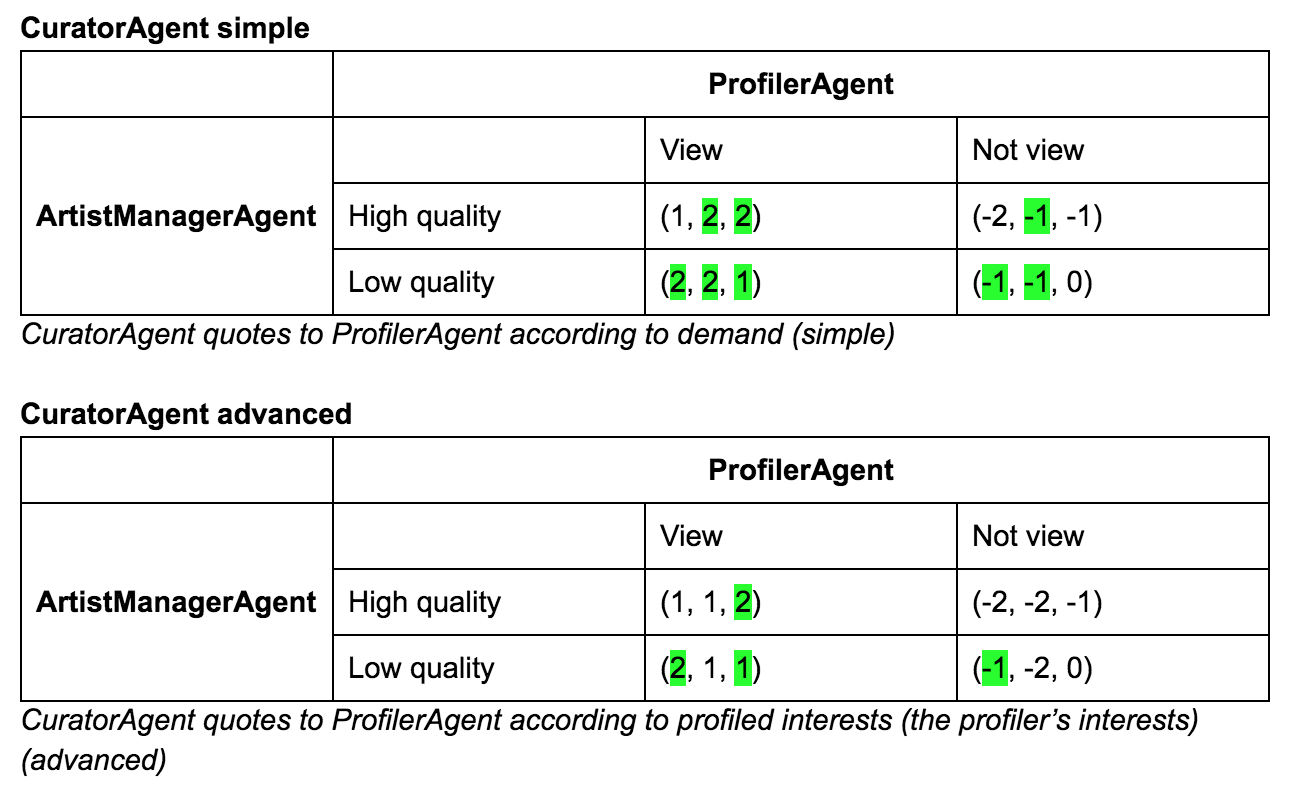
\includegraphics[width=1.0\linewidth]{payoff_matrices.png}
    \caption{Payoff matrix, with best decision (with respect to other agent's decisions) highlighted in green. The format of the payoff values is (ArtistManagerAgent, CuratorAgent, ProfilerAgent).}
    \label{fig:payoff_matrices}
\end{figure}

\subsubsection{Finding the Nash equilibrium}

We have a Nash equilibrium if each agent has chosen a strategy (i.e. made a decision, e.g. \texttt{ArtistManagerAgent} can choose between high quality and low quality) and all agents have chosen their optimal strategy with respect to the strategies the other agents chose.

To find the Nash equilibrium we take a look at the payoff matrix from the perspective of each agent. For every combination of choices the other agents can take, we find the optimal choice that we can make. If a cell in the payoff matrix only contains optimal choices (by all agents) then the set of strategies (decisions) and payoffs that that cell represents is a Nash equilibrium.

Let's look at the matrix from the \texttt{AristManagerAgent's} perspective. We fix the \texttt{CuratorAgent's} decision as \textit{simple} and the \texttt{ProfilerAgent's} decision as \textit{view}. We then decide what we would choose, we can choose \textit{high quality} with a payoff of 1 or \textit{low quality} with a payoff of 2, so we choose \textit{low quality}. The chosen value is highlighted in green in figure \ref{fig:payoff_matrices}.

Then we move on to the next combination of decisions that the other agents can take. We keep the \texttt{CuratorAgent's} decision fixed as \textit{simple}, and fix the \texttt{ProfilerAgent's} decision as \textit{not view}. We can then choose between a payoff of -2 for \textit{high quality} and -1 for \textit{low quality}, so we choose \textit{low quality}. We make a note of this choice (marking it as green in figure \ref{fig:payoff_matrices}) and move on to the next combination of decisions the other agents can make.

We repeat this process for all agents; going through all the combinations of decisions the other agents can make and finding our optimal decision in each case. After doing that we check if some cell in the payoff matrix contains only optimal decisions (by every agent). In figure \ref{fig:payoff_matrices} we can see that the cell for \[\textit{low quality, simple, view}\] contains only optimal decisions, so this set of decisions and payoffs constitutes a Nash equilibrium. This is the only Nash equilibrium available.

\end{document}
